\newcommand{\chapter}[2][]{
	\newcommand{\chapname}{#2}
	\begin{flushleft}
		\begin{minipage}[t]{\linewidth}
			
\includegraphics[height=1cm]{hdht-logo.png}
			\hspace{0pt}	
			\sffamily\bfseries\large Bài  9.
			\begin{flushleft}
				\LARGE\bfseries #1
			\end{flushleft}
		\end{minipage}
	\end{flushleft}
	\vspace{1cm}
	\normalfont\normalsize
}
\chapter[Chuyển động thẳng biến đổi đều:\\ đồ thị vận tốc - thời gian]{Chuyển động thẳng biến đổi đều: \\đồ thị vận tốc - thời gian}
\section{Lý thuyết}
\subsection{Phương trình chuyển động của chuyển động thẳng biến đổi đều}
Phương trình chuyển động của vật là phương trình mô tả sự thay đổi tọa độ của vật theo thời gian. 


Xét một điểm chuyển động thẳng biến đổi đều trên đường thẳng O$x$. Ở thời điểm ban đầu ($t_0$), chất điểm ở vị trí A có tọa độ $x_{0}$  với vận tốc ban đầu $v_0$ và gia tốc $a$. Mốc thời gian được chọn lúc bắt đầu chuyển động. Ở thời điểm $t$, chất điểm ở vị trí B có tọa độ $x$ như hình vẽ.  	
\begin{center}
	\begin{tikzpicture}
		\coordinate (laxis) at (-0.5,0);
		\coordinate (O) at (0,0);
		\coordinate (A) at (2,0);
		\coordinate (va) at ($(A)+(1,0)$);
		\coordinate (raxis) at (8,0);
		\coordinate (ldaxis) at (-0.5,-1);
		\coordinate (Od) at (0,-1);
		\coordinate (Ad) at (2,0);
		\coordinate (B) at (5,-1);
		\coordinate (vb) at ($(B)+(2,0)$);
		\coordinate (rdaxis) at (8,-1);
		\draw[->] (laxis) -- (raxis);
		\draw[->] (ldaxis) -- (rdaxis);
		
		
		\draw[->,ultra thick,blue] (A) -- (va);
		\draw[->,ultra thick,green!60!black] (B) -- (vb);
		\node[above=2mm] at (A) {A};
		\node[below left=1mm and 0.5mm] at (A) {$x_0$};
		\node[above=2mm] at (B) {B};
		\node[below left=1mm and 0.5mm] at (B) {$x$};
		\node[above=2mm] at (O) {O};
		
%		\node[above=2mm] at (Od) {O};
%		\node[below=2mm] at (C) {C};
		\node[right] at (raxis) {$x$};
		\node[above=1mm] at (va) {$\vec{v}_{0}$};
		\node[above=1mm] at (vb) {$\vec{v}$};
		
		\node[left=3cm,anchor=west] at (laxis) {thời điểm $t_0$};
		\node[left=3cm,anchor=west] at (ldaxis) {thời điểm $t> t_0$};
		\foreach \i in {O,Od,B,A}
			{
				\filldraw (\i) circle (2pt);
			}
		
%		\coordinate (odd) at ($(O)-(0,2)$);
		\coordinate (add) at ($(A)-(0,2)$);
		\coordinate (bdd) at ($(B)-(0,1)$);
%		\draw[<->,thick] (odd) -- (add);
		\draw[<->] (add) -- (bdd) node[midway,fill=pagecol] {$s$};
		\draw[dashed] (O)--(Od);
		\draw[dashed] (A)--(add);
		\draw[dashed] (B)--(bdd);
		
 	\end{tikzpicture}
\end{center}
Phương trình chuyển động của chất điểm có dạng 
	\begin{equation*}
		x=x_0+s=x_0+v_0(t-t_0)+\dfrac{1}{2}a(t-t_0)^2.
	\end{equation*}
Thông thường, để thuận tiện trong tính toán, ta chọn thời điểm $t_0=0$, khi đó phương trình chuyển động của chất điểm trở thành 
	\begin{equation*}
		x=x_0+v_0t+\dfrac{1}{2}at^{2}.
	\end{equation*}
\subsection {Phương trình vận tốc}
Nếu chất điểm bắt đầu chuyển động ở thời điểm $t_0$, thì phương trình vận tốc của chất điểm có dạng 
\begin{equation*}
	v=v_0+a(t-t_0)\quad \textrm{ với }t\geq t_0,
\end{equation*}

Vận tốc $v$ phụ thuộc thời gian theo hàm bậc nhất nên đồ thị vận tốc - thời gian có dạng là một nửa đường thẳng (do thời gian không âm) giới hạn bởi điểm ($t_0$, $x_0$). Như vậy:
\begin{itemize}
	\item Nếu gia tốc $a>0$ thì đồ thị hướng lên trên;
	\item Nếu gia tốc $a<0$ đồ thị hướng xuống dưới.
\end{itemize}

	\begin{figure}[h]
		\centering
		\begin{subfigure}{0.4\textwidth}
			\centering
			\begin{tikzpicture}
				\coordinate (O) at (0,0);
				\coordinate (xaxis) at (5,0);
				\coordinate (ydaxis) at (0,-2);
				\coordinate (yuaxis) at (0,2);
				\draw[->,name path=Ox] (O)--(xaxis);
				\draw[->,name path=Oy] (ydaxis)--(yuaxis);
				\node[below left] at (O) {O};
				\node[above] at (yuaxis) {$v$ };
				\node[right] at (xaxis) {$t$ };
				\path (0,-1.5) coordinate (vo) node[left] {$v_0$};
				\path (4,1.5) coordinate (v) node[left] {};
				\draw[thick,blue,name path=line] (vo)--(v);
				\node[above,text width=2.5cm,align=center] (1) at (2,1.5) {\small{nhanh dần đều }\\$a\cdot v>0$};
				\draw[->] (1.south) to [bend right] (2.7,0.8);
				\node[below,text width=1.5cm,align=center] (2) at (3.5,0) {\small{dừng lại}\\$v=0$};
				\path [name intersections={of=Ox and line,by=E}];
				\filldraw[red] (E) circle (2pt);
				\draw[->] (2.west) to [bend left] (2.05,-0.1);
				\node[below,text width=2.5cm,align=center] (3) at (3.5,-1.5) {\small{chậm dần đều}\\$a\cdot v<0$};
				\draw[->] (3.west) to [bend left] (1,-1);
			\end{tikzpicture}
			\caption*{\bfseries Đồ thị hướng lên trên: $a>0$}
		\end{subfigure}
		\hspace{1cm}
		\begin{subfigure}{0.4\textwidth}
			\centering
			\begin{tikzpicture}
				\coordinate (O) at (0,0);
				\coordinate (xaxis) at (5,0);
				\coordinate (ydaxis) at (0,-2);
				\coordinate (yuaxis) at (0,2);
				\draw[->,name path=Ox] (O)--(xaxis);
				\draw[->,name path=Oy] (ydaxis)--(yuaxis);
				\node[below left] at (O) {O};
				\node[above] at (yuaxis) {$v$ };
				\node[right] at (xaxis) {$t$ };
				\path (0,1.5) coordinate (vo) node[left] {$v_0$};
				\path (4,-1.5) coordinate (v) node[left] {};
				\draw[thick,blue,name path=line] (vo)--(v);
				\node[above,text width=2.5cm,align=center] (1) at (2.5,1.5) {\small{nhanh dần đều }\\$a\cdot v>0$};
				\draw[->] (1.south) to [bend left] (1.2,0.8);
				\node[below,text width=1.2cm,align=center] (2) at (0.8,0) {\small{dừng lại}\\$v=0$};
				\path [name intersections={of=Ox and line,by=E}];
				\filldraw[red] (E) circle (2pt);
				\draw[->] (2.east) to [bend right] (2,-0.1);
				\node[below,text width=2.5cm,align=center] (3) at (1.2,-1.5) {\small{chậm dần đều}\\$a\cdot v<0$};
				\draw[->] (3.east) to [bend right] (3,-1);
			\end{tikzpicture}
			\caption*{\bfseries Đồ thị hướng xuống dưới: $a<0$}
		\end{subfigure}
	\end{figure}
	
%	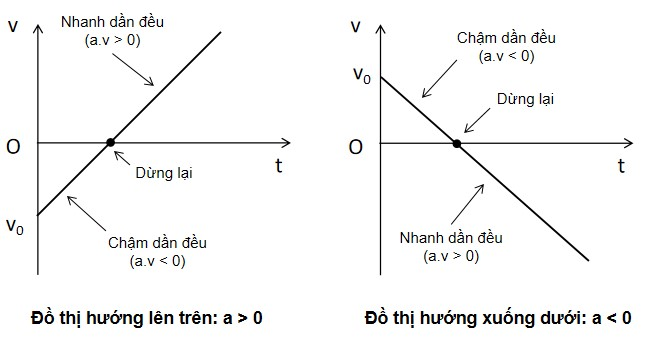
\includegraphics[scale=0.8]{../figs/VN10-PH-04-L-003-3-V2-01.jpg}


\section{Mục tiêu bài học - Ví dụ minh họa}
\begin{dang}{Xây dựng đồ thị vận tốc - thời gian, \\lập bảng giá trị tương ứng của \\ chuyển động thẳng biến đổi đều}
	\viduii{3}{
		Một vật chuyển động có đồ thị vận tốc như hình vẽ. Công thức vận tốc và công thức đường đi của vật là
		\begin{center}
			\begin{tikzpicture}
				\coordinate (O) at (0,0);
				\coordinate (xaxis) at (3.5,0);
				\coordinate (yaxis) at (0,3);
				\draw[->] (O)--(xaxis);
				\draw[->] (O)--(yaxis);
				\node[below left] at (O) {O};
				\node[above] at (yaxis) {$v$ (m/s)};
				\node[right] at (xaxis) {$t$ (s)};
				\path (0,1) coordinate (vo) node[left] {20};
				\coordinate (v) at ($(vo)+(30:3)$);
				\coordinate (vt) at ($(vo)+(30:2)$);
				\draw[thick,blue] (vo)--(v);
				\path let \p1=(vt) in (\x1,0) coordinate (vtx) node[below] {20};
				\path let \p1=(vt) in (0,\y1) coordinate (vty) node[left] {40};
				\draw[dashed] (vt)--(vtx);
				\draw[dashed] (vt)--(vty); 
			\end{tikzpicture}
		\end{center}
		\begin{mcq}(2)
			\item $v=t$, $s=\dfrac{1}{2}t^2$.
			\item $v=20+t$, $s=20t+\dfrac{1}{2}t^2$.
			\item $v=20-t$, $s=20t-\dfrac{1}{2}t^2$.
			\item $v=40-2t$, $s=40t-\dfrac{1}{2}t^2$.
		\end{mcq}
	}
	{	\begin{center}
			\textbf{Hướng dẫn giải}
		\end{center}
		Đồ thị vận tốc - thời gian có dạng đường thẳng với hệ số góc khác không nên đây là đồ thị mô tả chuyển động thẳng biến đổi đều. 
		
		Gia tốc của vật được tính theo công thức
		\begin{equation*}
			a=\dfrac{v-v_0}{t}=\dfrac{\SI{40}{\meter/\second}-\SI{20}{\meter/\second}}{\SI{20}{\second}}=\SI{1}{\meter/\second^2}.
		\end{equation*}
		
		Phương trình vận tốc có dạng 
		\begin{equation*}
			v=v_0+at=20+t\textrm{ (m/s, s)}.
		\end{equation*}
		
		Công thức tính quãng đường đi được 
		\begin{equation*}
			s=v_0 t+\dfrac{1}{2}at^2=20t+\dfrac{1}{2}t^2\textrm{ (m, s)}.
		\end{equation*}
		
		\textbf{Đáp án: B}.
	}
	\viduii{3}{Một xe đạp đang chuyển động với vận tốc $\SI{5}{\meter/\second}$ thì hãm phanh chuyển động chậm dần đều có đồ thị vận tốc theo thời gian sau. Tính quãng đường đi được từ lúc hãm phanh cho đến khi dừng lại.
		
		\begin{center}
				\begin{tikzpicture}
					\coordinate (O) at (0,0);
					\coordinate (xaxis) at (4,0);
					\coordinate (yaxis) at (0,3);
					\draw[->] (O)--(xaxis);
					\draw[->] (O)--(yaxis);
					\node[below left] at (O) {O};
					\node[above] at (yaxis) {$v$ (m/s)};
					\node[right] at (xaxis) {$t$ (s)};
					\path (0,2) coordinate (vo) node[left] {5};
					\path (3,0) coordinate (v) node[below] {10};
					\draw[thick,blue] (vo)--(v);
				\end{tikzpicture}
		\end{center}
	}
	{	\begin{center}
			\textbf{Hướng dẫn giải}
		\end{center}
		
		Gia tốc của vật là
		\begin{equation*}
			a=\dfrac{v-v_0}{t}=\dfrac{0-\SI{5}{\meter/\second}}{\SI{10}{\second}}=-\SI{0.5}{\meter/\second^2}.
		\end{equation*}
		
		Quãng đường đi được từ lúc hãm phanh cho đến khi dừng lại là:
		\begin{equation*}
			v^2-v_0^2=2as\quad\Rightarrow\quad  s=\dfrac{v^2-v_0^2}{2a}=\dfrac{(\SI{0}{\meter/\second})^{2}-(\SI{5}{\meter/\second})^2}{2\cdot (\SI{-0.5}{\meter/\second^2})}=\SI{25}{\meter}.
		\end{equation*}
	}
	\viduii{3}{Đồ thị vận tốc thời gian của một vật chuyển động như hình vẽ bên.
		\begin{center}
			\begin{tikzpicture}[scale=0.7]
				\coordinate (O) at (0,0);
				\coordinate (xaxis) at (7,0);
				\coordinate (yaxis) at (0,4);
				\draw[->] (O)--(xaxis);
				\draw[->] (O)--(yaxis);
				\node[below left] at (O) {O};
				\node[left] at (yaxis) {$v$ (m/s)};
				\node[right] at (xaxis) {$t$ (s)};
				\coordinate (A) at (0,2);
				\coordinate (B) at (1,3);
				\coordinate (C) at (3,3);
				\coordinate (D) at (6,0);				\node[right] at  (A) {A};
				\node[above] at (B) {B};
				\node[above] at (C) {C};
				\node[above right] at (D) {D};
				\draw[thick,blue] (A)--(B)--(C)--(D);
				\path let \p1=(B) in (\x1,0) coordinate (bd) node[below] {10};
				\path let \p2=(C) in (\x2,0) coordinate (cd) node[below] {30};
				\path let \p3=(B) in (0,\y3) coordinate (bl) node[left] {15};
				\node[left] at (A) {10};
				\node[below] at (D) {60};
				\draw[dashed] (B)--(bd);
				\draw[dashed] (C)--(cd);
				\draw[dashed] (B)--(bl);
			\end{tikzpicture}
%			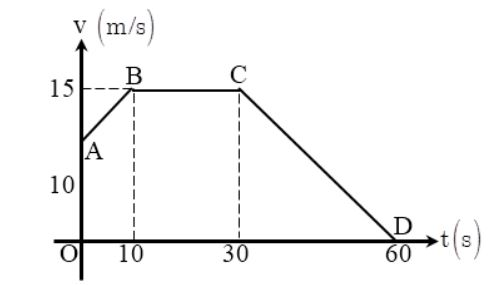
\includegraphics[scale=0.8]{../figs/VN10-PH-04-L-003-3-V2-04.jpg}
		\end{center}
		\begin{enumerate}[label=\alph*.]
			\item Nêu tính chất chuyển động của mỗi giai đoạn? 
			\item Lập phương trình vận tốc của mỗi giai đoạn?
		\end{enumerate}
		
	}
	{	\begin{center}
			\textbf{Hướng dẫn giải}
		\end{center}
		
		\begin{enumerate}[label=\alph*.]
			\item Tính chất chuyển động của mỗi giai đoạn:
				\begin{description}
					\item[AB] chuyển động nhanh dần đều do đồ thị thể hiện vận tốc tăng với hệ số góc không đổi.
					\item[BC] chuyển động thẳng đều do đồ thị thể hiện vận tốc không thay đổi theo thời gian.
					\item[CD] chuyển động chậm dần đều đến khi dừng lại do đồ thị thể hiện vận tốc giảm đều về 0.
				\end{description}
			\item Phương trình vận tốc của mỗi giai đoạn	
				\begin{align*}
					v_\text{AB}& = 10 +(\SI{0.5}{\meter/\second})\times t&(\SI{0}{\second}\leq t \leq \SI{10}{\second}),\\
					v_\text{BC} &= \SI{15}{m/s}.&(\SI{10}{\second}<t\leq \SI{30}{\second}),\\
					v_\text{CD} &= 15 - (\SI{0.5}{\meter/\second})\times t & (\SI{30}{\second} < t \leq \SI{60}{\second}).
				\end{align*}
		\end{enumerate}

	}
	
\end{dang}
